\Transcb{yellow}{blue}{Einstein's insight}
\onecolumn
\begin{itemize}
\item Einstein~: Observer in free fall to the earth $\rightarrow$ No experience of the gravitational field
\item[] $\rightarrow$ An accelerated frame can transform gravity away
\item[] Objects at rest close to the observer will stay at rest $\rightarrow$ Local inertial frame
\item[] $\rightarrow$ {\red The gravitational field has only a relative existence}
\item[$\ast$] Consequence~: {\blue Gravity can be induced by accelerating the reference frame}
\end{itemize}
%
\begin{center}
\raisebox{5cm}{\colorbox{yellow}{The equivalence principle}} \hspace*{2cm}
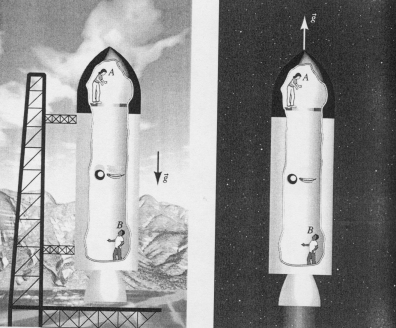
\includegraphics[keepaspectratio,height=10cm]{equivalence}
\end{center}
